\chapter{A New Section - Such as Related Work}
\label{cahp-rl}

Duis aliquam hendrerit nunc vitae euismod. Nam in laoreet ante. Vestibulum nec purus eget urna varius commodo luctus in lacus. Quisque eu nisl dui. Maecenas sagittis rutrum ante id imperdiet. Sed semper odio vel est bibendum commodo. Vivamus lacinia facilisis ante. Etiam venenatis at eros eu sollicitudin. Proin aliquet, neque in suscipit finibus, purus mi elementum est, finibus elementum libero turpis faucibus nibh. Proin orci arcu, euismod a lacinia vel, porta a turpis \cite{apples1}.

\section{The subsection -- about a Toolkit}

Praesent eget neque ac tortor finibus hendrerit et eu mauris. Nam quis finibus risus, ac tristique turpis. Curabitur non mauris eget sapien eleifend scelerisque lobortis eu lacus. Sed metus augue, volutpat id tristique in, ultrices in massa. Donec et dui in massa rhoncus scelerisque. Nunc luctus dui sed ullamcorper molestie. Phasellus efficitur nec est sit amet dignissim. In convallis orci ac urna maximus, et congue nisl lobortis.

\section{Internals of the toolkit}

Sed facilisis commodo leo, id interdum est. Vivamus ultricies pharetra tortor, nec imperdiet enim mattis non. Duis sagittis sem ut urna sodales semper. Vestibulum ullamcorper dui at libero faucibus vulputate at nec nulla. Fusce justo est, maximus eu commodo sed, sagittis dictum felis. Integer id velit ac ipsum volutpat bibendum. Nunc dictum pretium eros, tincidunt sodales enim porta a.

\begin{figure}[ht]
  \begin{center}
    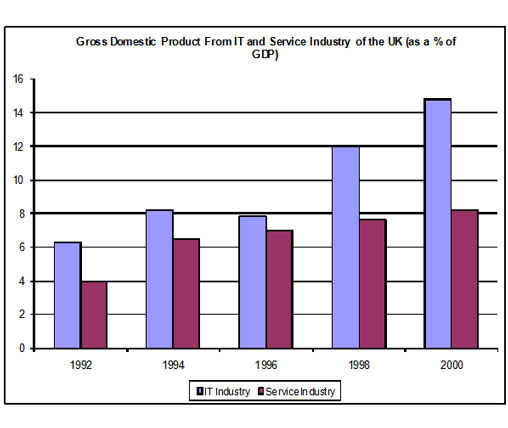
\includegraphics[scale=0.65]{Histogram}
    \caption{Some Bar Chart}
  \end{center}
\end{figure}

Another list can go like this, and more explanations can be added \cite{apples2}.
\begin{enumerate}
  \item
  Connectivity protocols 
  \item
  Resource protocols 
  \item
  Collective protocols 
\end{enumerate}

\section{Services and Technologies}
Vestibulum tempus ipsum in gravida hendrerit. Donec vehicula mi a rhoncus pellentesque. Morbi sit amet vestibulum tortor. Nulla facilisi. Nulla felis velit, accumsan maximus ornare sit amet, congue a dolor. Mauris quis pulvinar justo. Phasellus nec consequat tellus. Ut tempor venenatis risus. Nam sit amet mauris tincidunt leo porttitor tempor. Nam at urna ac leo fringilla accumsan. Morbi eu tristique ligula. Cras ut pellentesque orci. Orci varius natoque penatibus et magnis dis parturient montes, nascetur ridiculus mus. Duis suscipit nunc diam, vitae semper nibh maximus rhoncus. Donec pharetra elit viverra sapien elementum aliquet. Duis hendrerit quam elit, in pretium enim ultricies ac.

\subsection{An example for sub-sub-section}
Etiam risus ante, viverra vel diam sed, eleifend blandit quam. Vivamus quis gravida arcu. Fusce ac est ut velit maximus pellentesque vitae quis massa. Aenean eget tortor nisi. Phasellus hendrerit nibh sit amet dolor molestie interdum vel a lacus. Nam est leo, consequat id nibh ac, molestie facilisis velit. Cras at urna nisl.

\section{Programming Section}

Praesent in feugiat turpis, et laoreet turpis. Etiam lobortis, metus sit amet iaculis tincidunt, velit orci porta magna, vitae faucibus arcu orci nec justo. Morbi quis elit non massa tincidunt ornare ullamcorper quis mauris. Vivamus nec sollicitudin tortor, venenatis cursus mi. Donec at turpis non leo euismod hendrerit vulputate et tortor. Quisque malesuada lectus vitae orci condimentum sagittis. Nunc ut ligula a eros venenatis pretium

\begin{center}
  \begin{parbox}[t]{.45\linewidth}
    {\textsf{\underline{Sample Mathematical Explanation} \\
      (1) P $\xrightarrow{getPK(R)}$ GSM$_u$ \\
      1.1 $GSM_u$ $\xrightarrow{R}$ GSM$_R$\\
      1.2 $GSM_u$ $\xleftarrow{PK_R}$ GSM$_R$\\
      (2) P $\xleftarrow{PK_R}$ $GSM_u$ \\
      (3) P $\xrightarrow{C=Enc_{PK_R}(M)}$ R \\
      (4) P $\xleftarrow{M}$ R \\
      (5) P considers R authenticated \\
      \hfill
    }} \\
  \end{parbox}
\end{center}
